%%%%%%%%%%%%%%%%%%%%%%%%%%%%%%%%%%%%%%%%%%%%%%%%%%%%%%%%%%%%%%%%%%%%%%%%%%%%%%%%%%
\begin{frame}[fragile]\frametitle{}
\begin{center}
{\Large Agents using LangGraph}
\end{center}
\end{frame}

%%%%%%%%%%%%%%%%%%%%%%%%%%%%%%%%%%%%%%%%%%%%%%%%%%%%%%%%%%%
\begin{frame}[fragile]\frametitle{LangChain vs LangGraph}
\begin{columns}
    \begin{column}[T]{0.6\linewidth}
        \begin{center}
        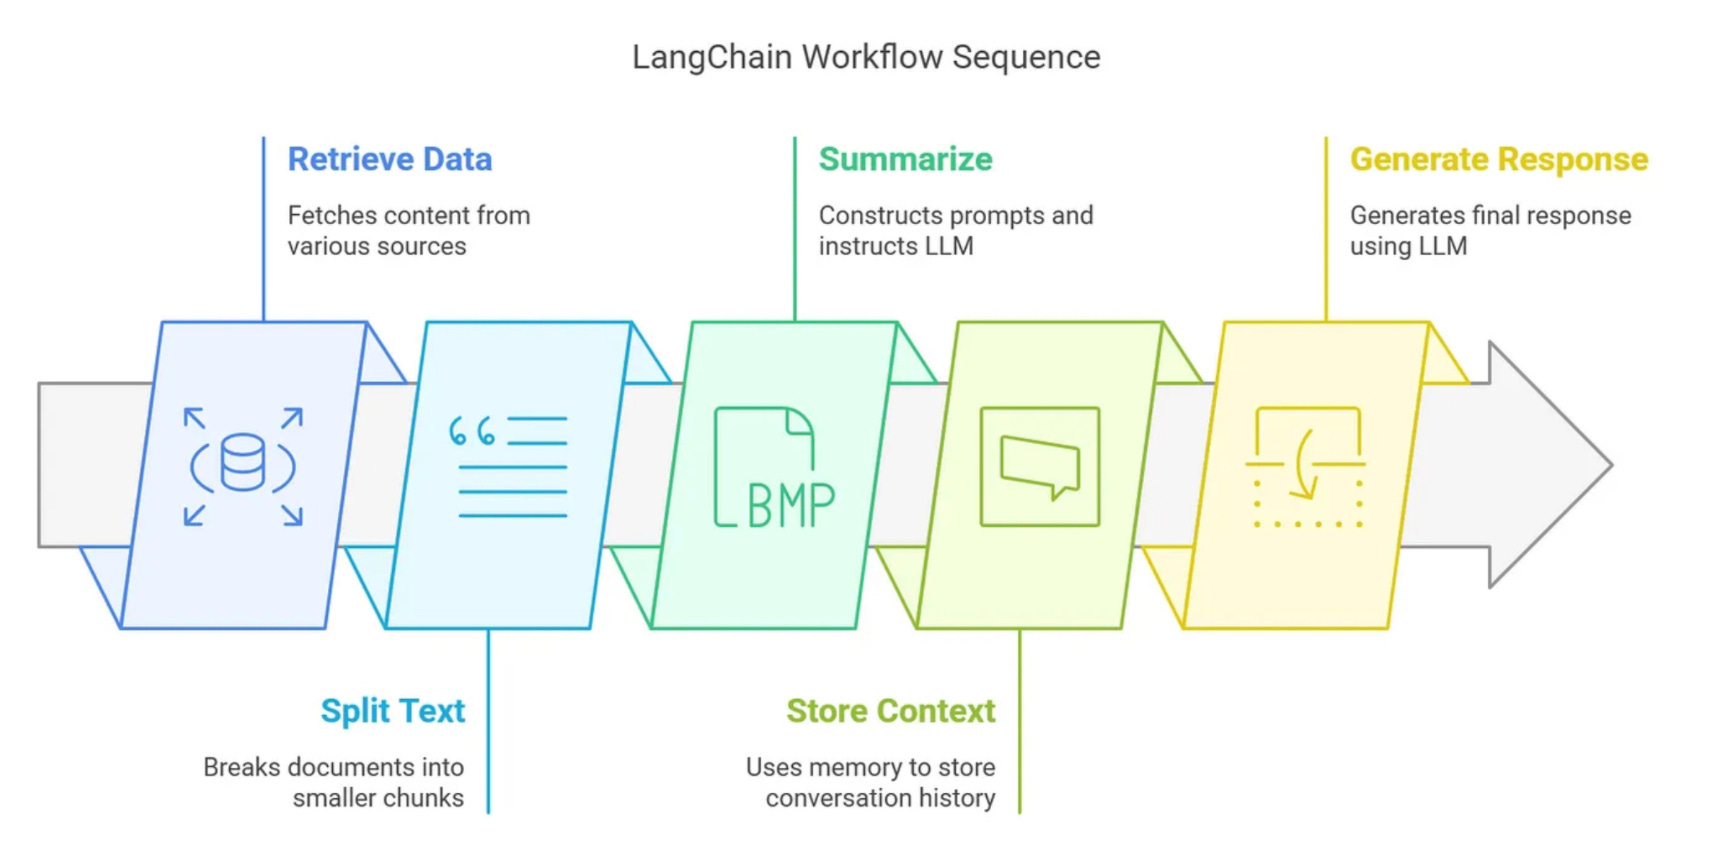
\includegraphics[width=0.8\linewidth,keepaspectratio]{aiagents64}
		
        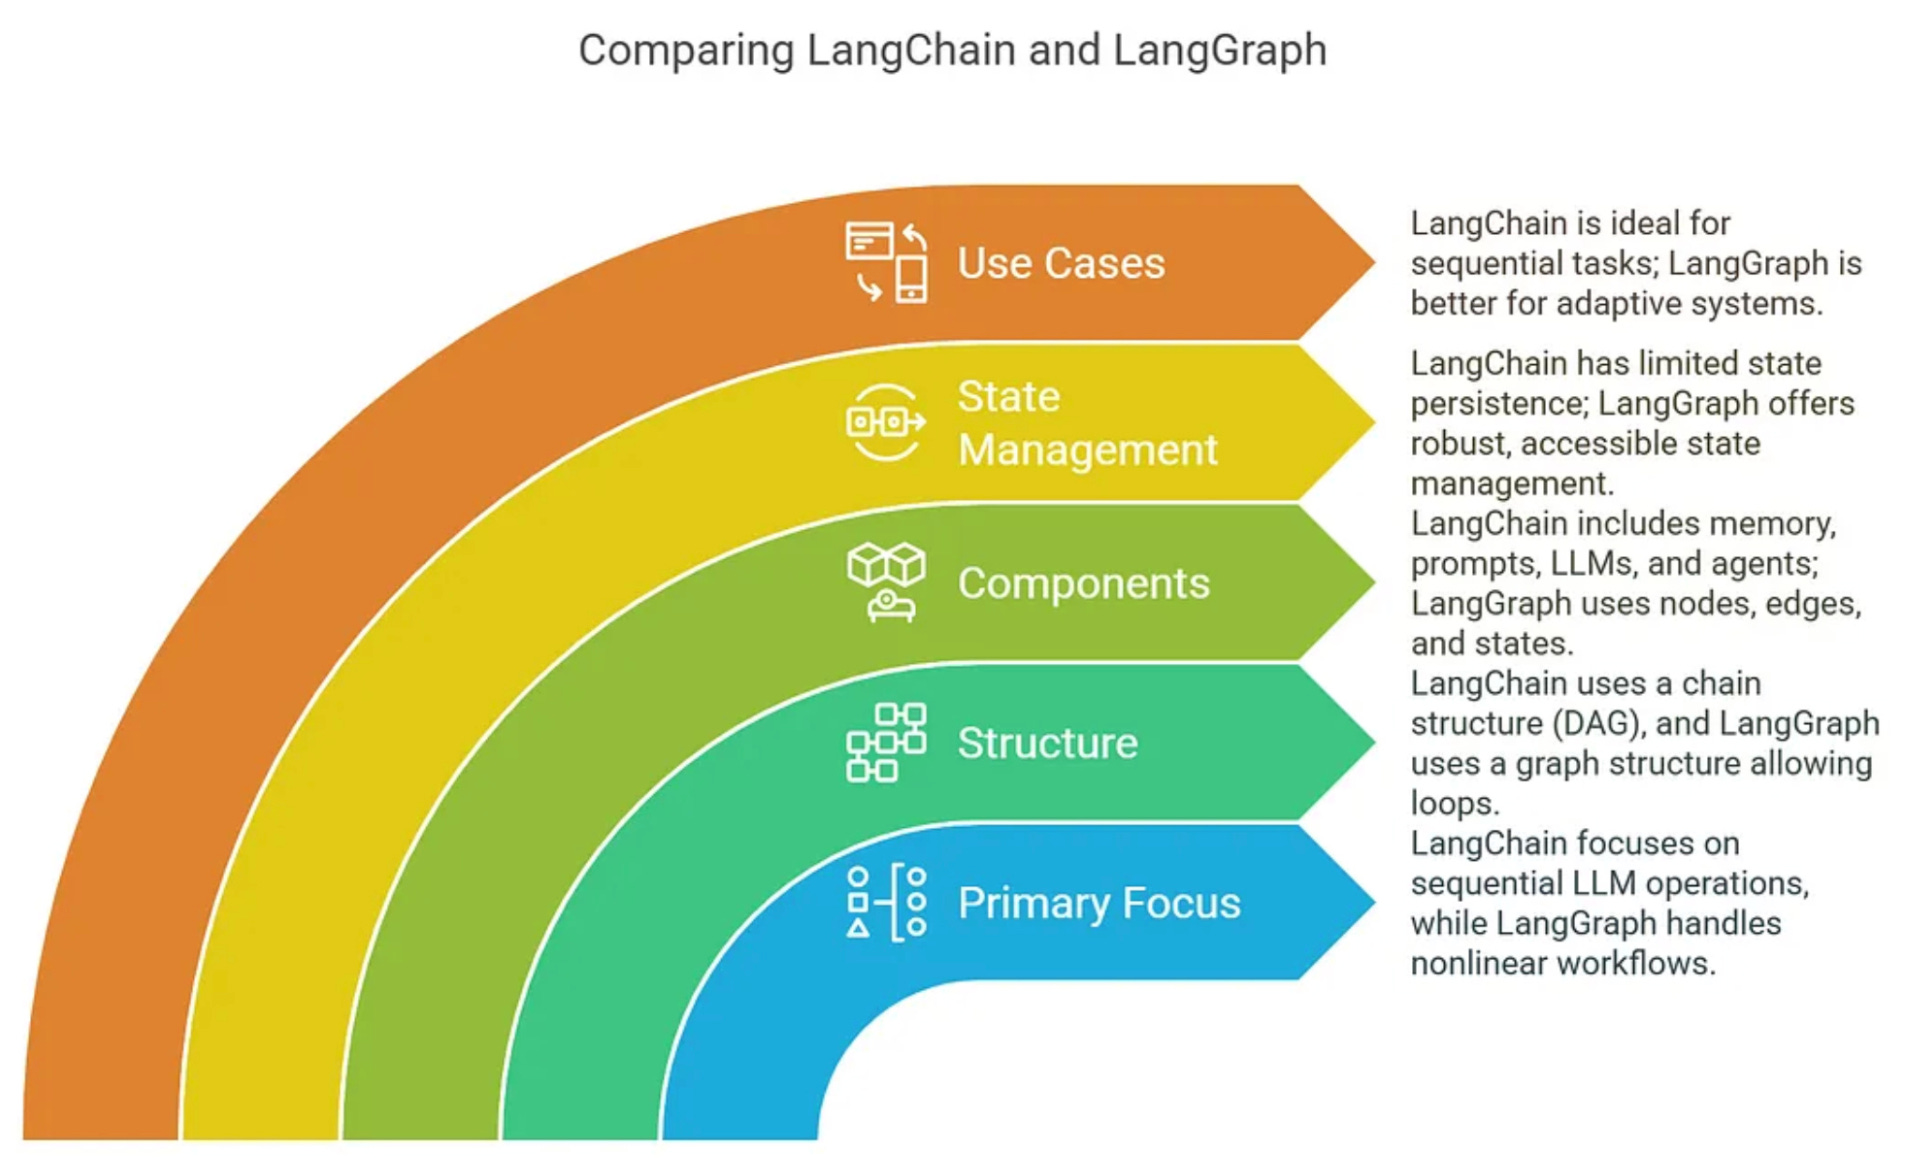
\includegraphics[width=0.8\linewidth,keepaspectratio]{aiagents66}
		
		{\tiny (Ref: Vizuara AI Agents Bootcamp)}
				
        \end{center}    
    \end{column}
    \begin{column}[T]{0.4\linewidth}
        \begin{center}
        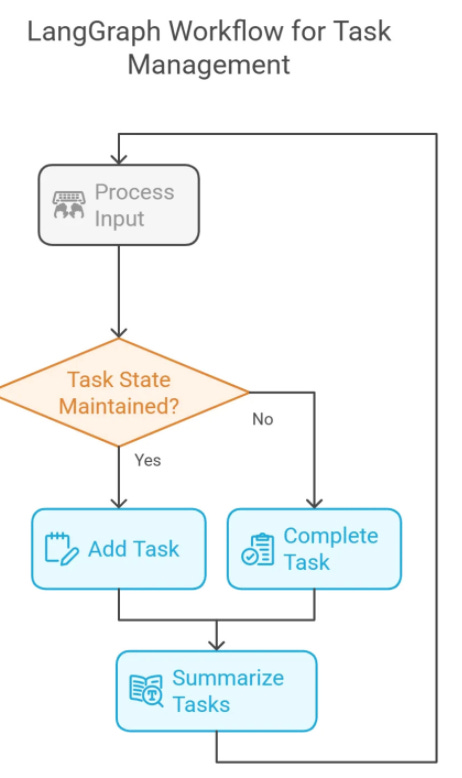
\includegraphics[width=0.8\linewidth,keepaspectratio]{aiagents65}
		
		{\tiny (Ref: Vizuara AI Agents Bootcamp)}
				
        \end{center}    
    \end{column}
  \end{columns}
\end{frame}


%%%%%%%%%%%%%%%%%%%%%%%%%%%%%%%%%%%%%%%%%%%%%%%%%%%%%%%%%%%
\begin{frame}[fragile]\frametitle{LangChain vs LangGraph – Why a New Approach?}

      \begin{itemize}
        \item LangChain excels at straightforward pipelines with fixed sequential tasks (retrieve → summarize → answer)
        \item Real-world workflows aren't always linear - they need branches, loops, and dynamic decision points
        \item LangGraph specializes in stateful, non-linear workflows within the LangChain ecosystem
        \item LangGraph exposes control flow explicitly, allowing fine-grained control over agent behavior
        \item You define a graph of possible steps instead of a rigid chain structure
        \item Agents can revisit nodes or choose different paths dynamically based on conditions
        \item Use LangChain for simple sequences, LangGraph for conditional logic and extended context
        \item LangGraph enables complex multi-agent systems with evolving task flows
      \end{itemize}

\end{frame}

%%%%%%%%%%%%%%%%%%%%%%%%%%%%%%%%%%%%%%%%%%%%%%%%%%%%%%%%%%%
\begin{frame}[fragile]\frametitle{LangGraph Fundamentals: Nodes, Edges \& State}

      \begin{itemize}
        \item \textbf{Nodes (N):} Individual processing steps implemented as Python functions that transform state
        \item Each node encapsulates one sub-task: LLM calls, calculations, file operations, or tool invocations
        \item \textbf{Edges (E):} Directed connections determining execution order and flow between nodes
        \item Edges can be linear progressions or conditional routes based on current state
        \item \textbf{State (S):} Shared data object (dictionary/TypedDict) persisting throughout agent execution
        \item State enables context and memory across workflow, allowing nodes to read previous results
        \item StateGraph ties everything together with designated START and END nodes
        \item This approach handles interactive, conditional loops that static chains struggle with
      \end{itemize}
  

\end{frame}

%%%%%%%%%%%%%%%%%%%%%%%%%%%%%%%%%%%%%%%%%%%%%%%%%%%%%%%%%%%
\begin{frame}[fragile]\frametitle{LangGraph}
\begin{columns}
    \begin{column}[T]{0.5\linewidth}
        \begin{center}
		
        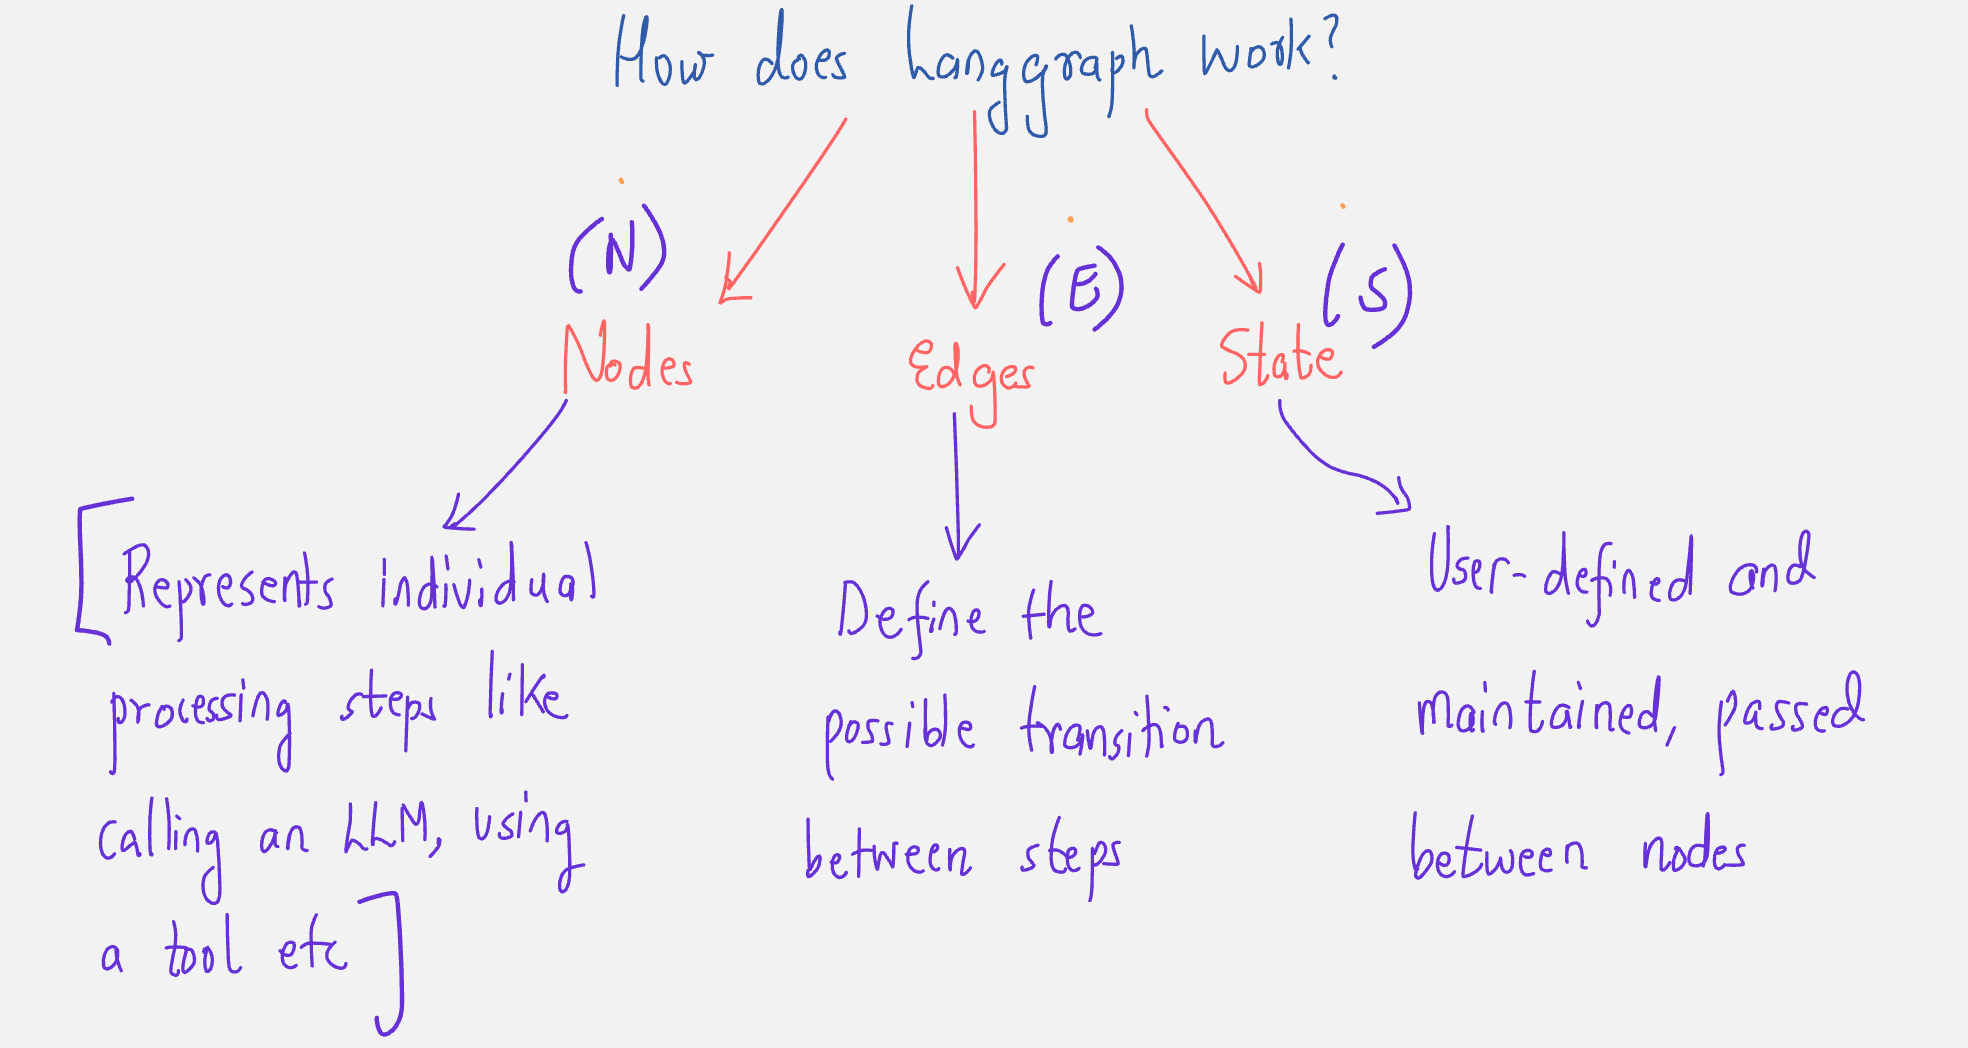
\includegraphics[width=0.8\linewidth,keepaspectratio]{aiagents67}
		
        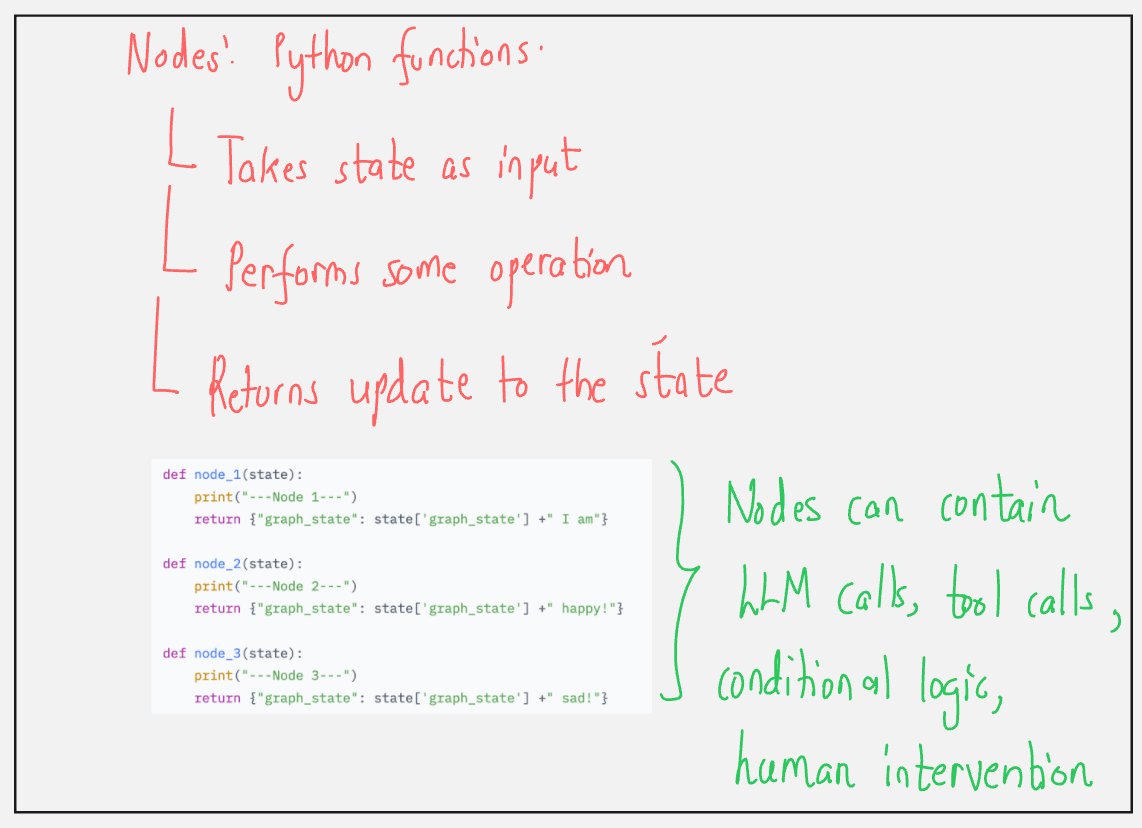
\includegraphics[width=0.8\linewidth,keepaspectratio]{aiagents68}
		
		
		{\tiny (Ref: Vizuara AI Agents Bootcamp)}
				
        \end{center}    
    \end{column}
    \begin{column}[T]{0.5\linewidth}
        \begin{center}
        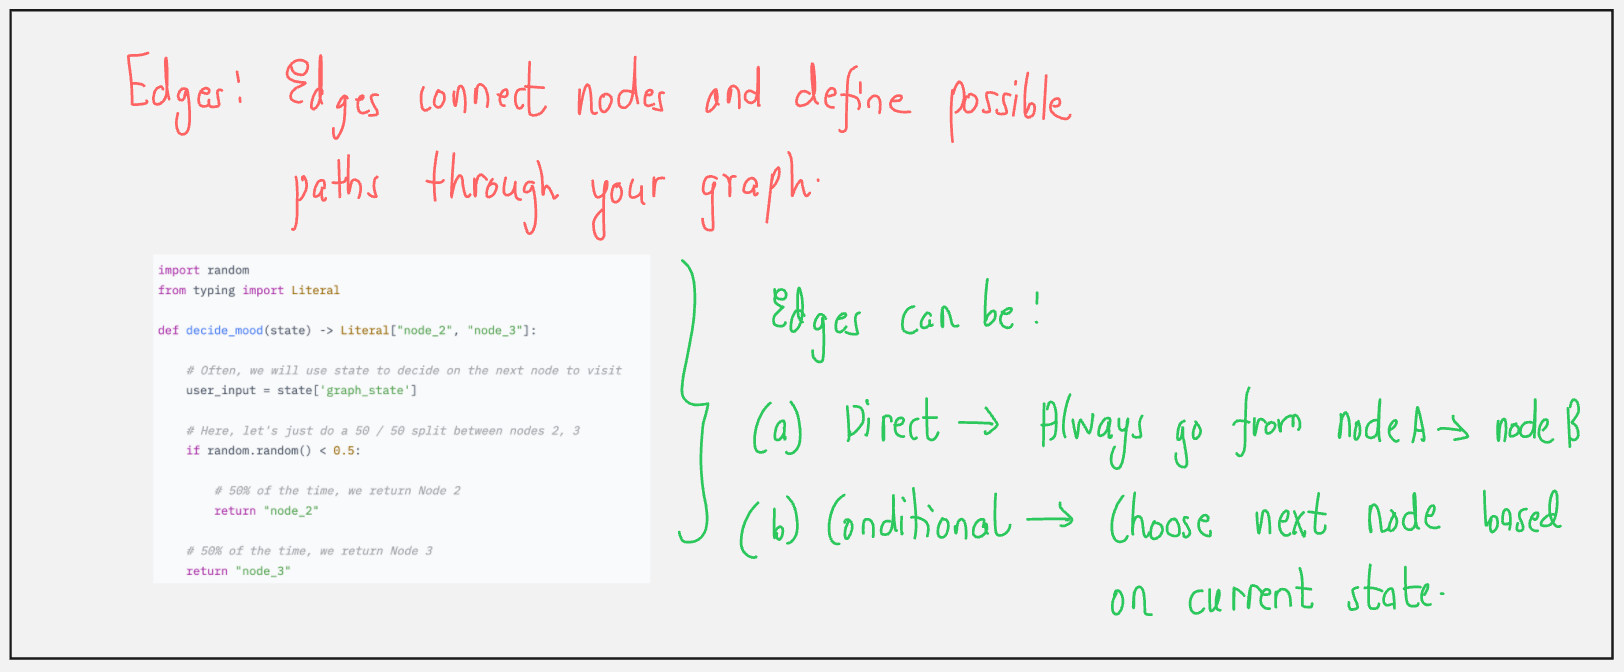
\includegraphics[width=0.8\linewidth,keepaspectratio]{aiagents69}
		
        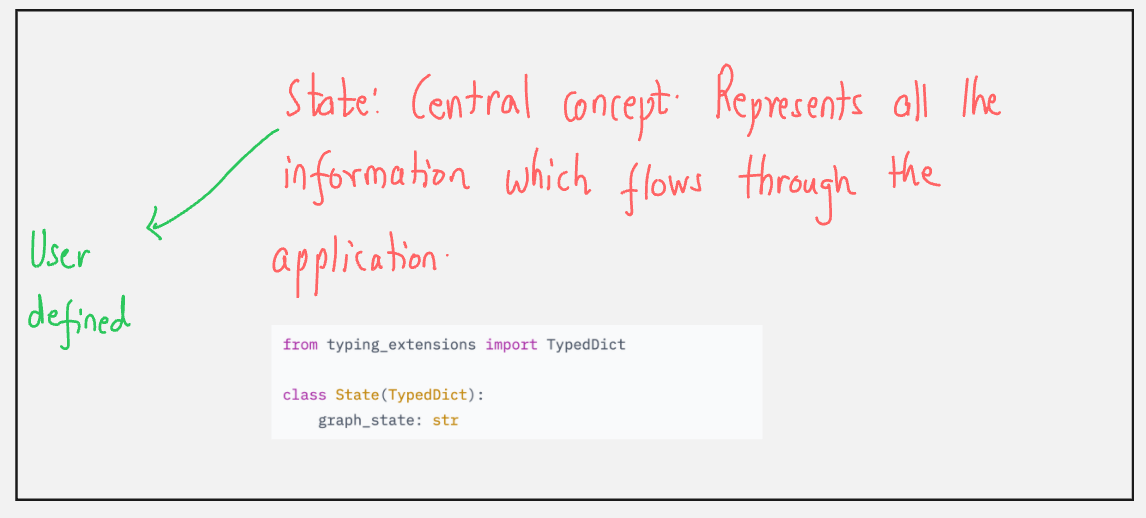
\includegraphics[width=0.8\linewidth,keepaspectratio]{aiagents70}
		
        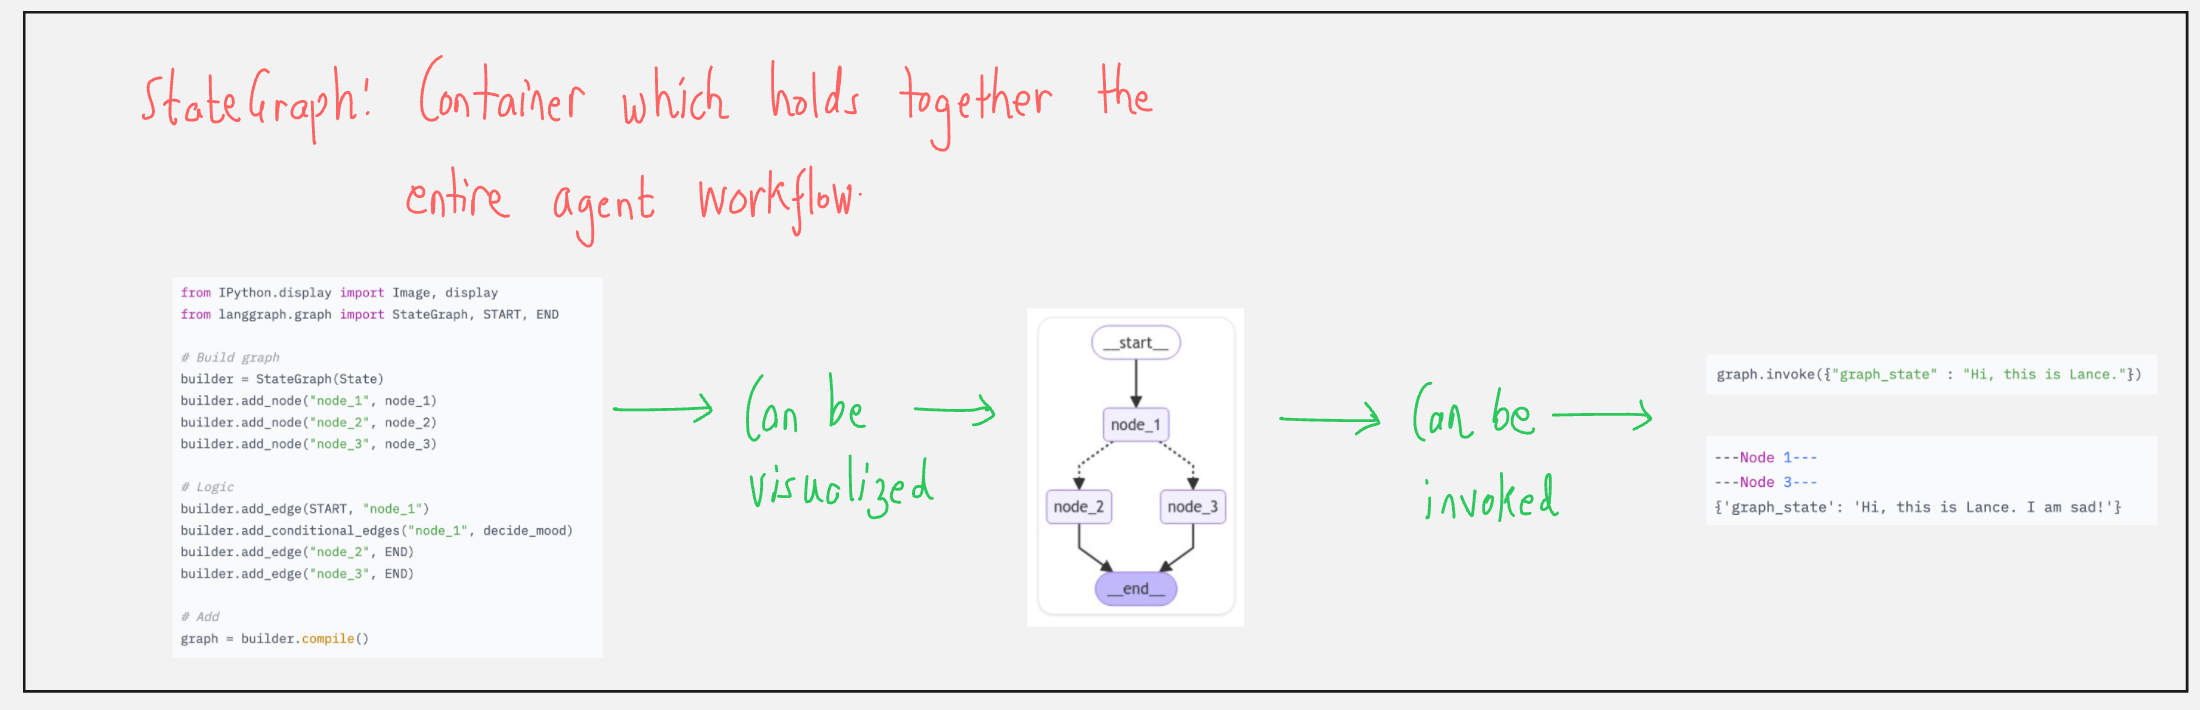
\includegraphics[width=0.8\linewidth,keepaspectratio]{aiagents71}
		
		{\tiny (Ref: Vizuara AI Agents Bootcamp)}
				
        \end{center}    
    \end{column}
  \end{columns}
\end{frame}

%%%%%%%%%%%%%%%%%%%%%%%%%%%%%%%%%%%%%%%%%%%%%%%%%%%%%%%%%%%
\begin{frame}[fragile]\frametitle{Building an Email Sorting Agent}

      \begin{itemize}
        \item Email processing assistant inspired by Alfred managing Bruce Wayne's inbox
        \item \textbf{EmailState:} Contains email content, spam flag, category, draft response, and message history
        \item \textbf{Five nodes:} read\_email → classify\_email → handle\_spam/drafting\_response → notify\_mr\_wayne
        \item Classify\_email uses LLM to analyze content and set spam status in state
        \item Conditional edge routes to spam handler or response drafter based on classification
        \item Handle\_spam terminates workflow early, drafting\_response continues to notification
        \item Demonstrates clear if/else logic through graph structure rather than buried code
        \item Successfully tested on legitimate and crypto spam emails with correct routing
      \end{itemize}

\end{frame}

%%%%%%%%%%%%%%%%%%%%%%%%%%%%%%%%%%%%%%%%%%%%%%%%%%%%%%%%%%%
\begin{frame}[fragile]\frametitle{LangGraph}
\begin{columns}
    \begin{column}[T]{0.5\linewidth}
        \begin{center}
	
        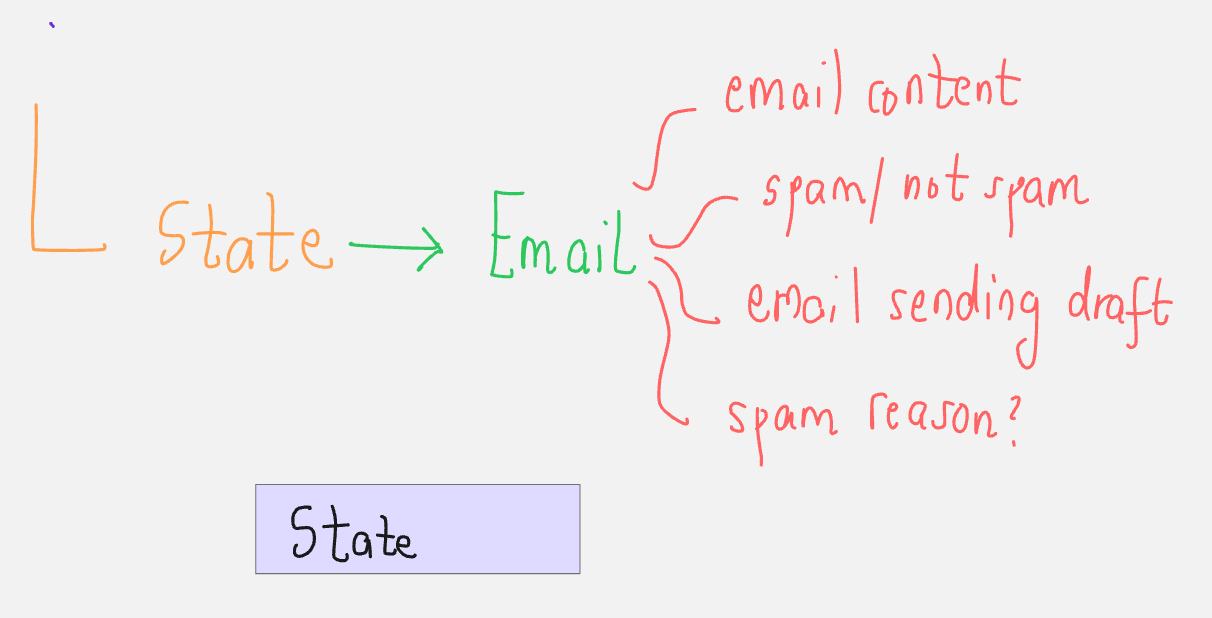
\includegraphics[width=0.8\linewidth,keepaspectratio]{aiagents72}
	
        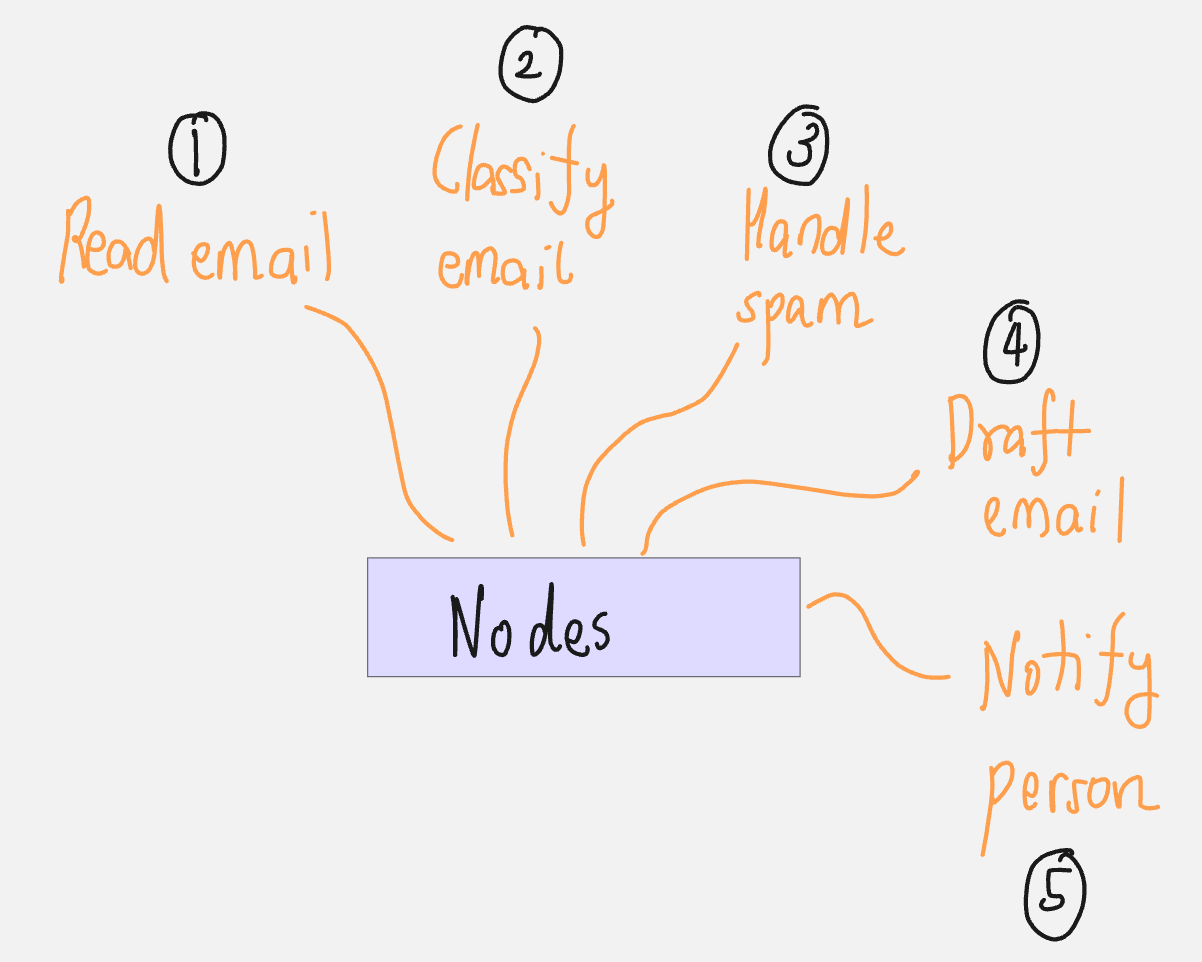
\includegraphics[width=0.8\linewidth,keepaspectratio]{aiagents73}
		
		{\tiny (Ref: Vizuara AI Agents Bootcamp)}
				
        \end{center}    
    \end{column}
    \begin{column}[T]{0.5\linewidth}
        \begin{center}

        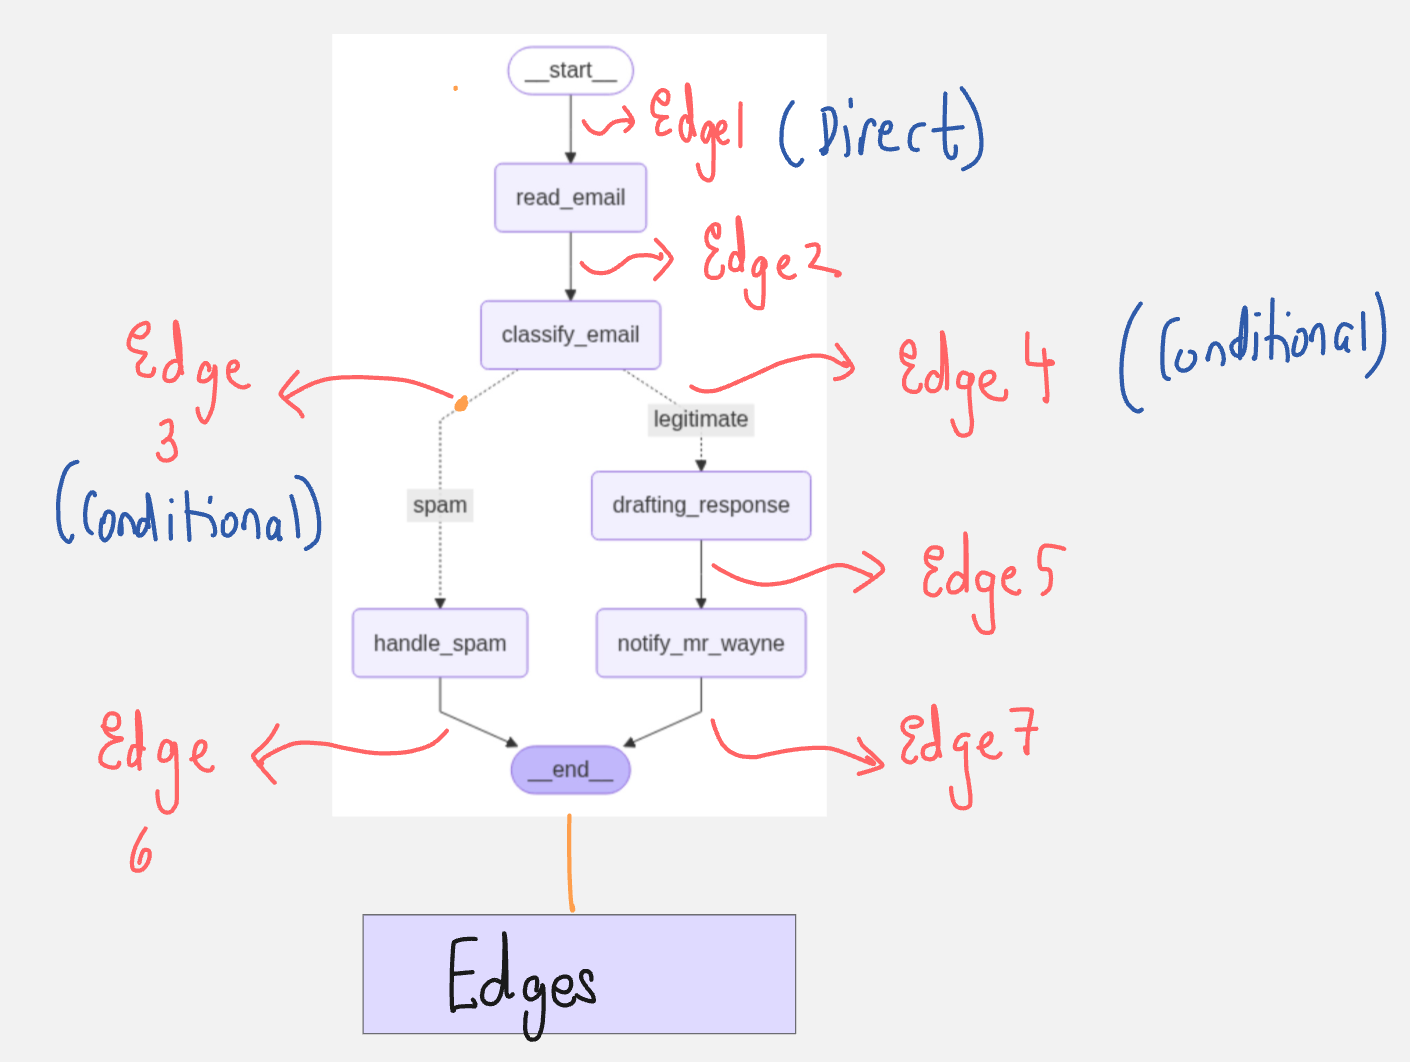
\includegraphics[width=0.8\linewidth,keepaspectratio]{aiagents74}
		
		{\tiny (Ref: Vizuara AI Agents Bootcamp)}
				
        \end{center}    
    \end{column}
  \end{columns}
\end{frame}

%%%%%%%%%%%%%%%%%%%%%%%%%%%%%%%%%%%%%%%%%%%%%%%%%%%%%%%%%%%
\begin{frame}[fragile]\frametitle{LangGraph}

        \begin{center}

        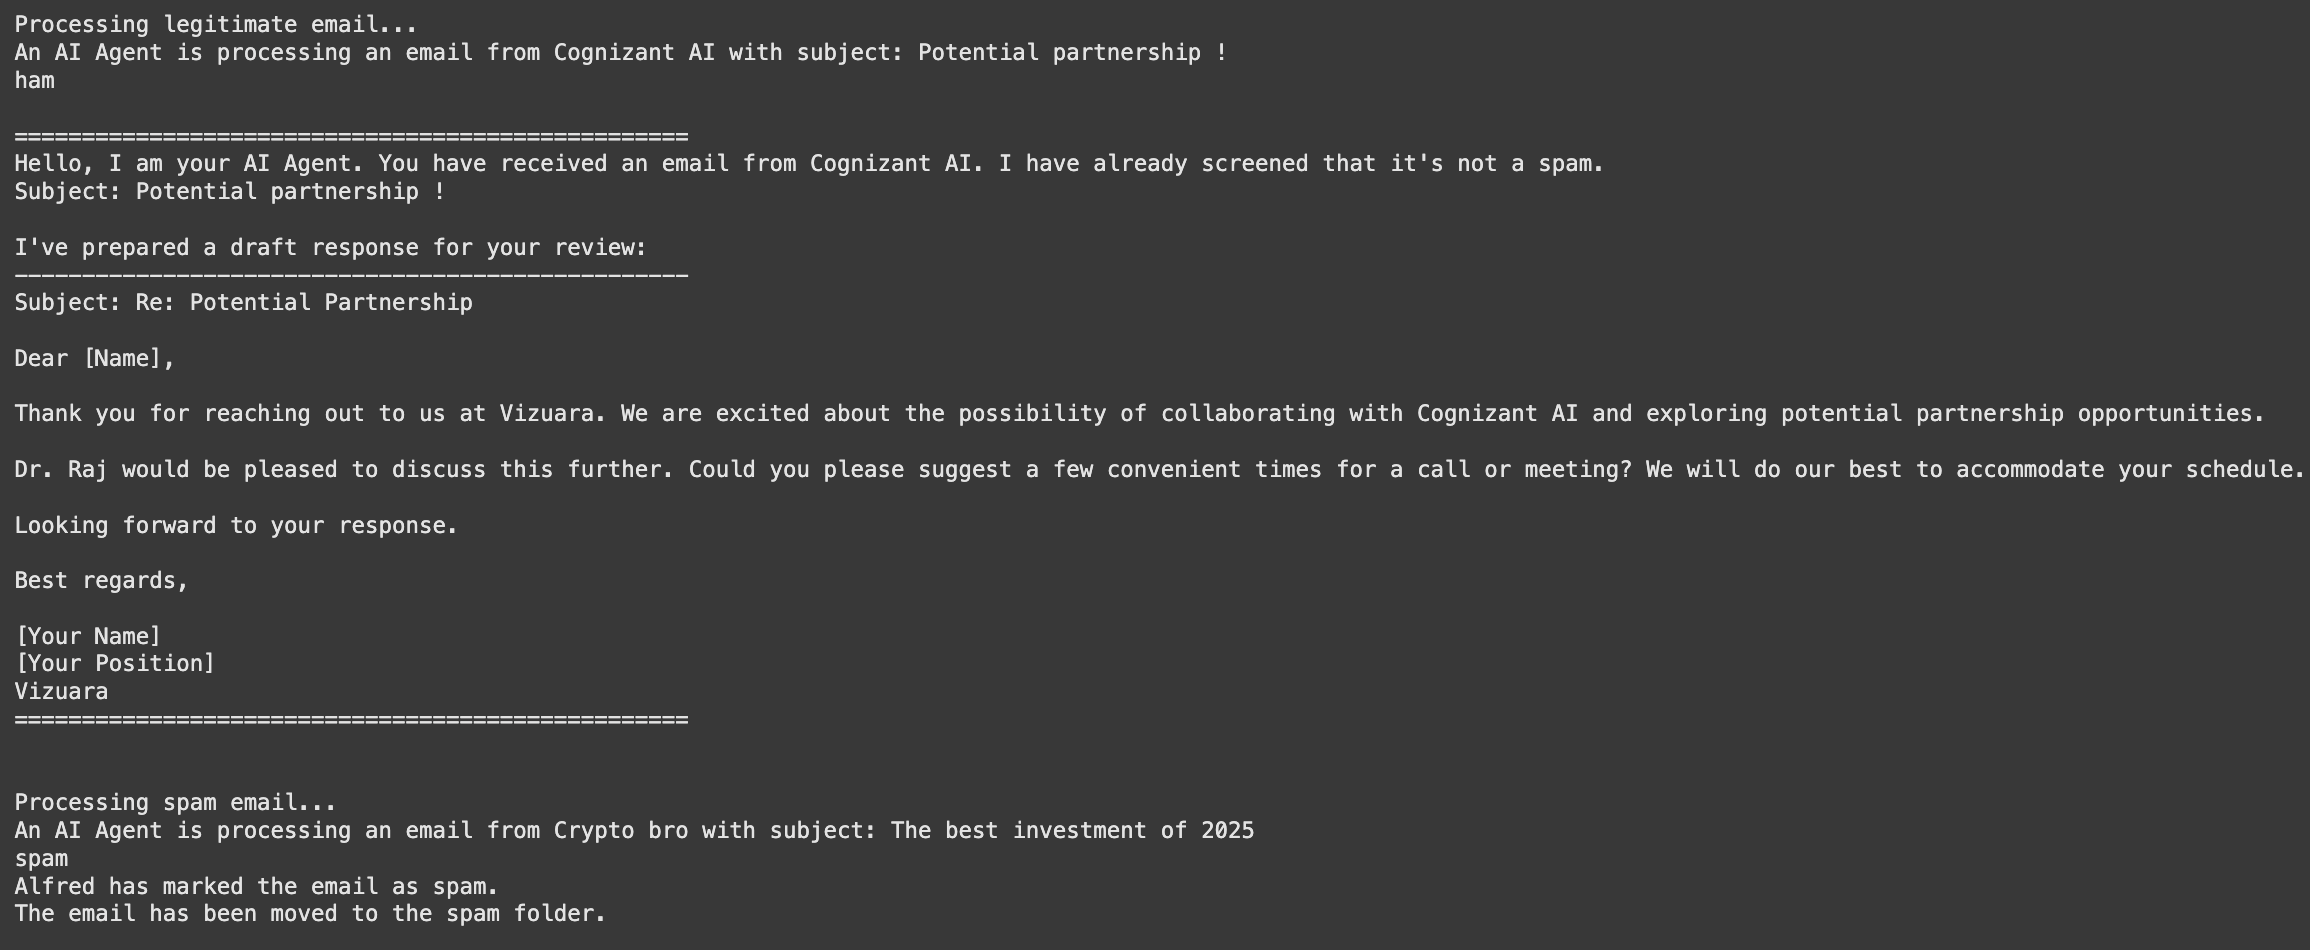
\includegraphics[width=\linewidth,keepaspectratio]{aiagents75}
		
		{\tiny (Ref: Vizuara AI Agents Bootcamp)}
				
        \end{center}    

\end{frame}

%%%%%%%%%%%%%%%%%%%%%%%%%%%%%%%%%%%%%%%%%%%%%%%%%%%%%%%%%%%
\begin{frame}[fragile]\frametitle{Creating a Vision Assistant Agent}
\begin{columns}
    \begin{column}[T]{0.7\linewidth}
      \begin{itemize}
        \item Vision-enabled agent implementing explicit "Thought → Action → Observation" loop
        \item \textbf{AgentState:} Stores input\_file (image path) and messages list for conversation history
        \item \textbf{Assistant node:} GPT-4 with vision capability bound to image analysis and math tools
        \item \textbf{Tools node:} Executes tool functions (extract\_text, divide) and records results
        \item Assistant decides to use tools or provide final answer based on task requirements
        \item Conditional edge uses tools\_condition to route between assistant and tools nodes
        \item Creates cycle: assistant thinks → tool execution → assistant processes results → repeat
        \item Loop continues until assistant provides final answer without requesting tools
      \end{itemize}
    \end{column}
    \begin{column}[T]{0.3\linewidth}
        \begin{center}
        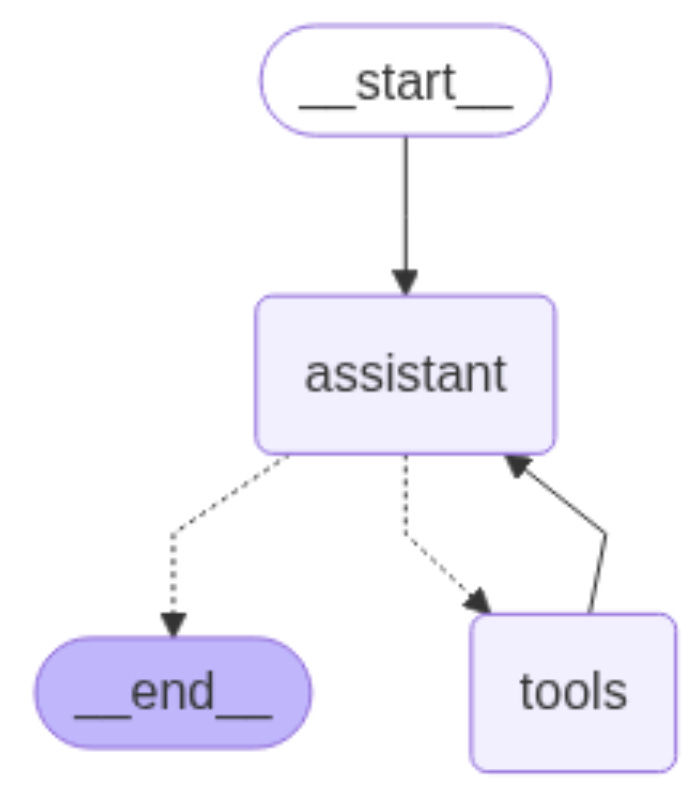
\includegraphics[width=\linewidth,keepaspectratio]{aiagents76}
        \end{center}    
    \end{column}
  \end{columns}
\end{frame}

%%%%%%%%%%%%%%%%%%%%%%%%%%%%%%%%%%%%%%%%%%%%%%%%%%%%%%%%%%%
\begin{frame}[fragile]\frametitle{Creating a Vision Assistant Agent}

        \begin{center}

        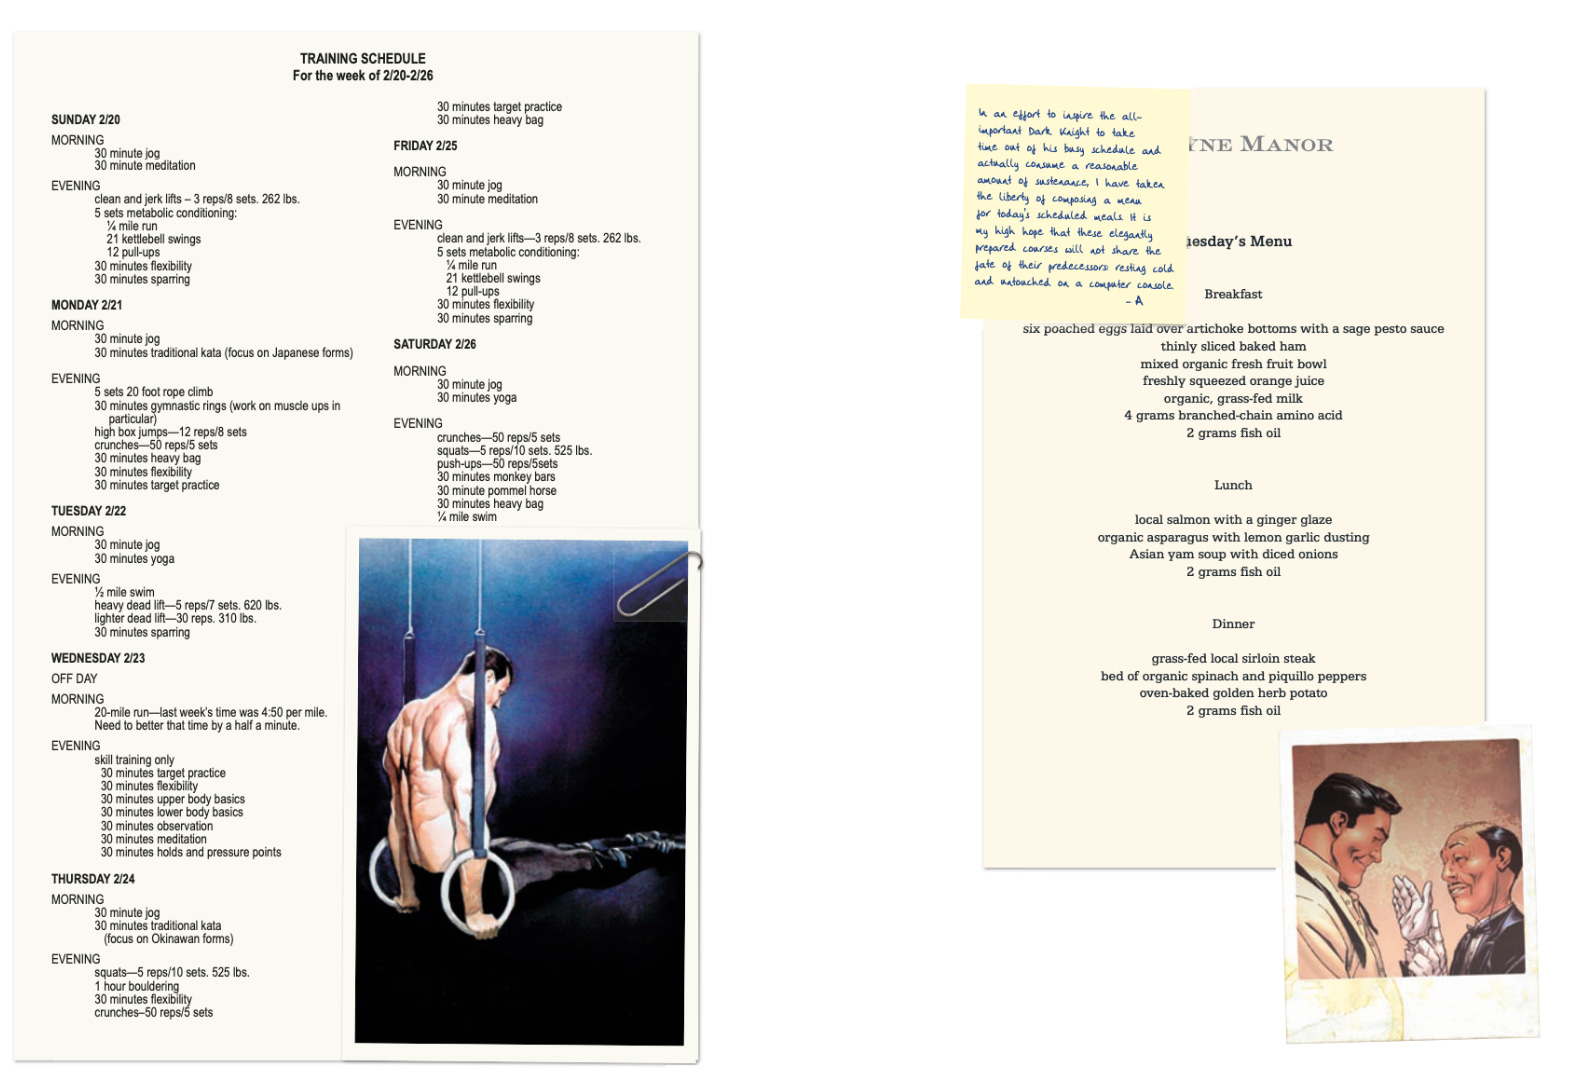
\includegraphics[width=0.9\linewidth,keepaspectratio]{aiagents77}
		
		{\tiny (Ref: Vizuara AI Agents Bootcamp)}
				
        \end{center}    

\end{frame}

%%%%%%%%%%%%%%%%%%%%%%%%%%%%%%%%%%%%%%%%%%%%%%%%%%%%%%%%%%%
\begin{frame}[fragile]\frametitle{Creating a Vision Assistant Agent}

        \begin{center}

        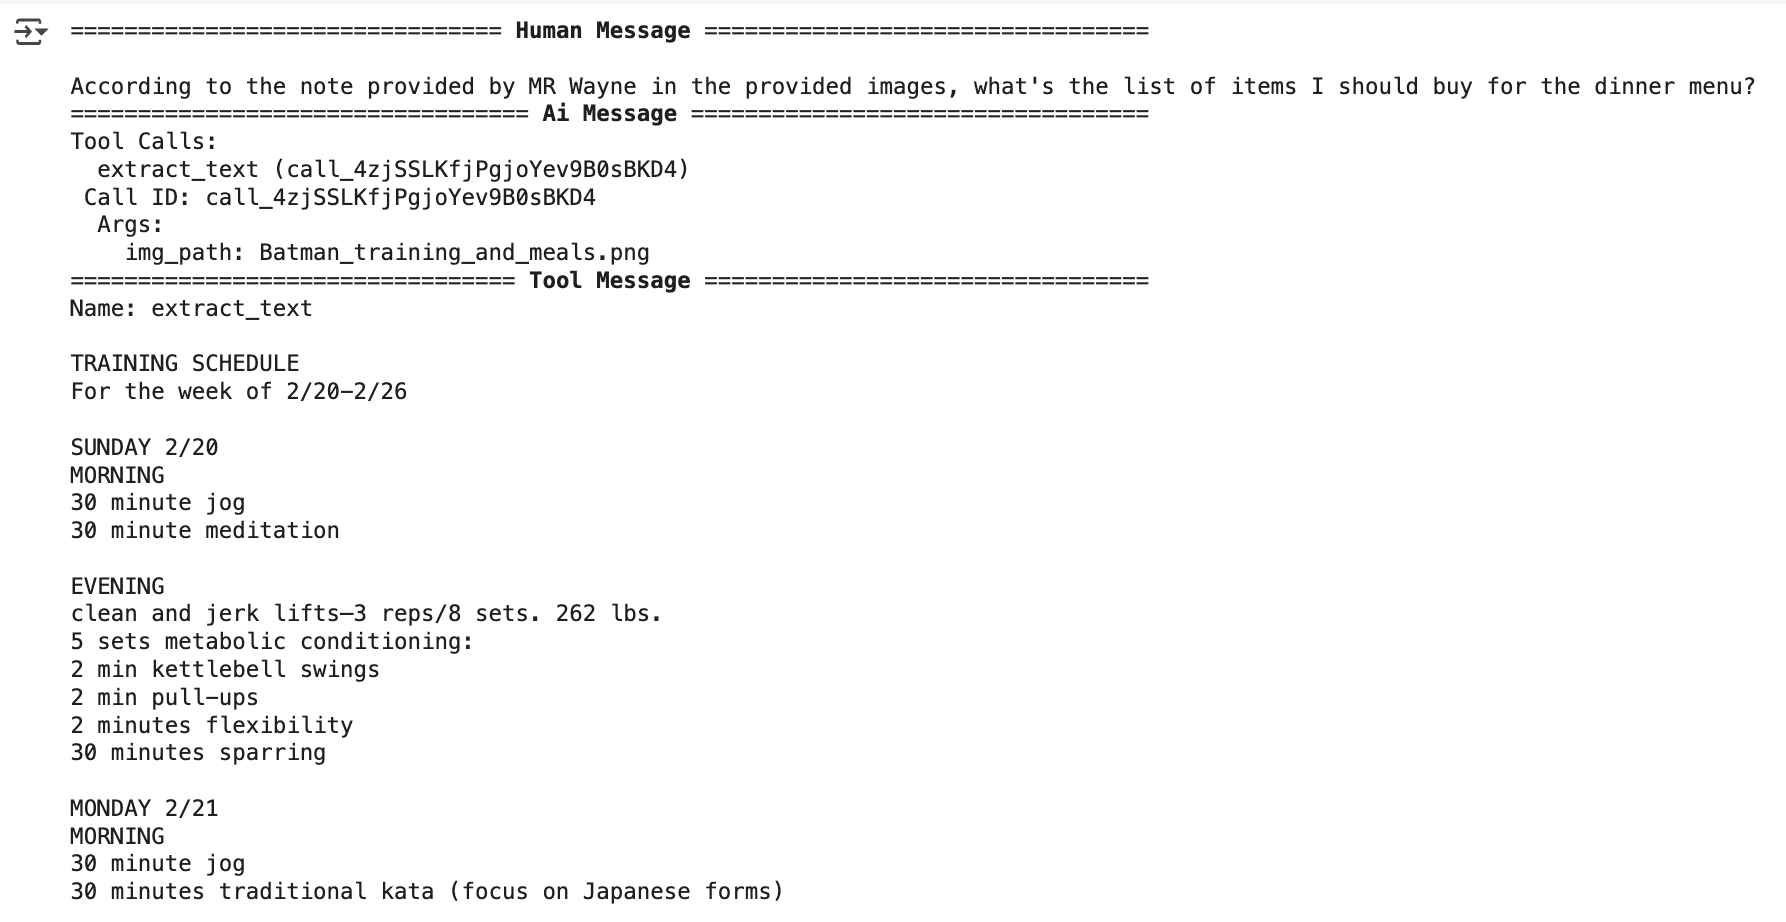
\includegraphics[width=\linewidth,keepaspectratio]{aiagents78}
		
		{\tiny (Ref: Vizuara AI Agents Bootcamp)}
				
        \end{center}    

\end{frame}



%%%%%%%%%%%%%%%%%%%%%%%%%%%%%%%%%%%%%%%%%%%%%%%%%%%%%%%%%%%
\begin{frame}[fragile]\frametitle{Tracing Agent Workflows with Langfuse}

      \begin{itemize}
        \item Observability crucial for debugging complex agent behaviors with multiple steps
        \item \textbf{Traces:} Detailed execution records capturing prompts, responses, paths, and tool usage
        \item Langfuse provides user-friendly dashboard for inspecting agent workflow traces
        \item Integrates via OpenTelemetry standards with tracing callbacks in LangGraph code
        \item Enables monitoring of both email agent and vision agent execution flows
        \item Tools-assistant loop clearly visible in Langfuse trace visualization
        \item Answers "why did my agent do X?" through accessible trace inspection
        \item Essential best practice for moving from prototypes to production-grade AI systems
      \end{itemize}

\end{frame}

%%%%%%%%%%%%%%%%%%%%%%%%%%%%%%%%%%%%%%%%%%%%%%%%%%%%%%%%%%%
\begin{frame}[fragile]\frametitle{Tracing Agent Workflows with Langfuse}

        \begin{center}

        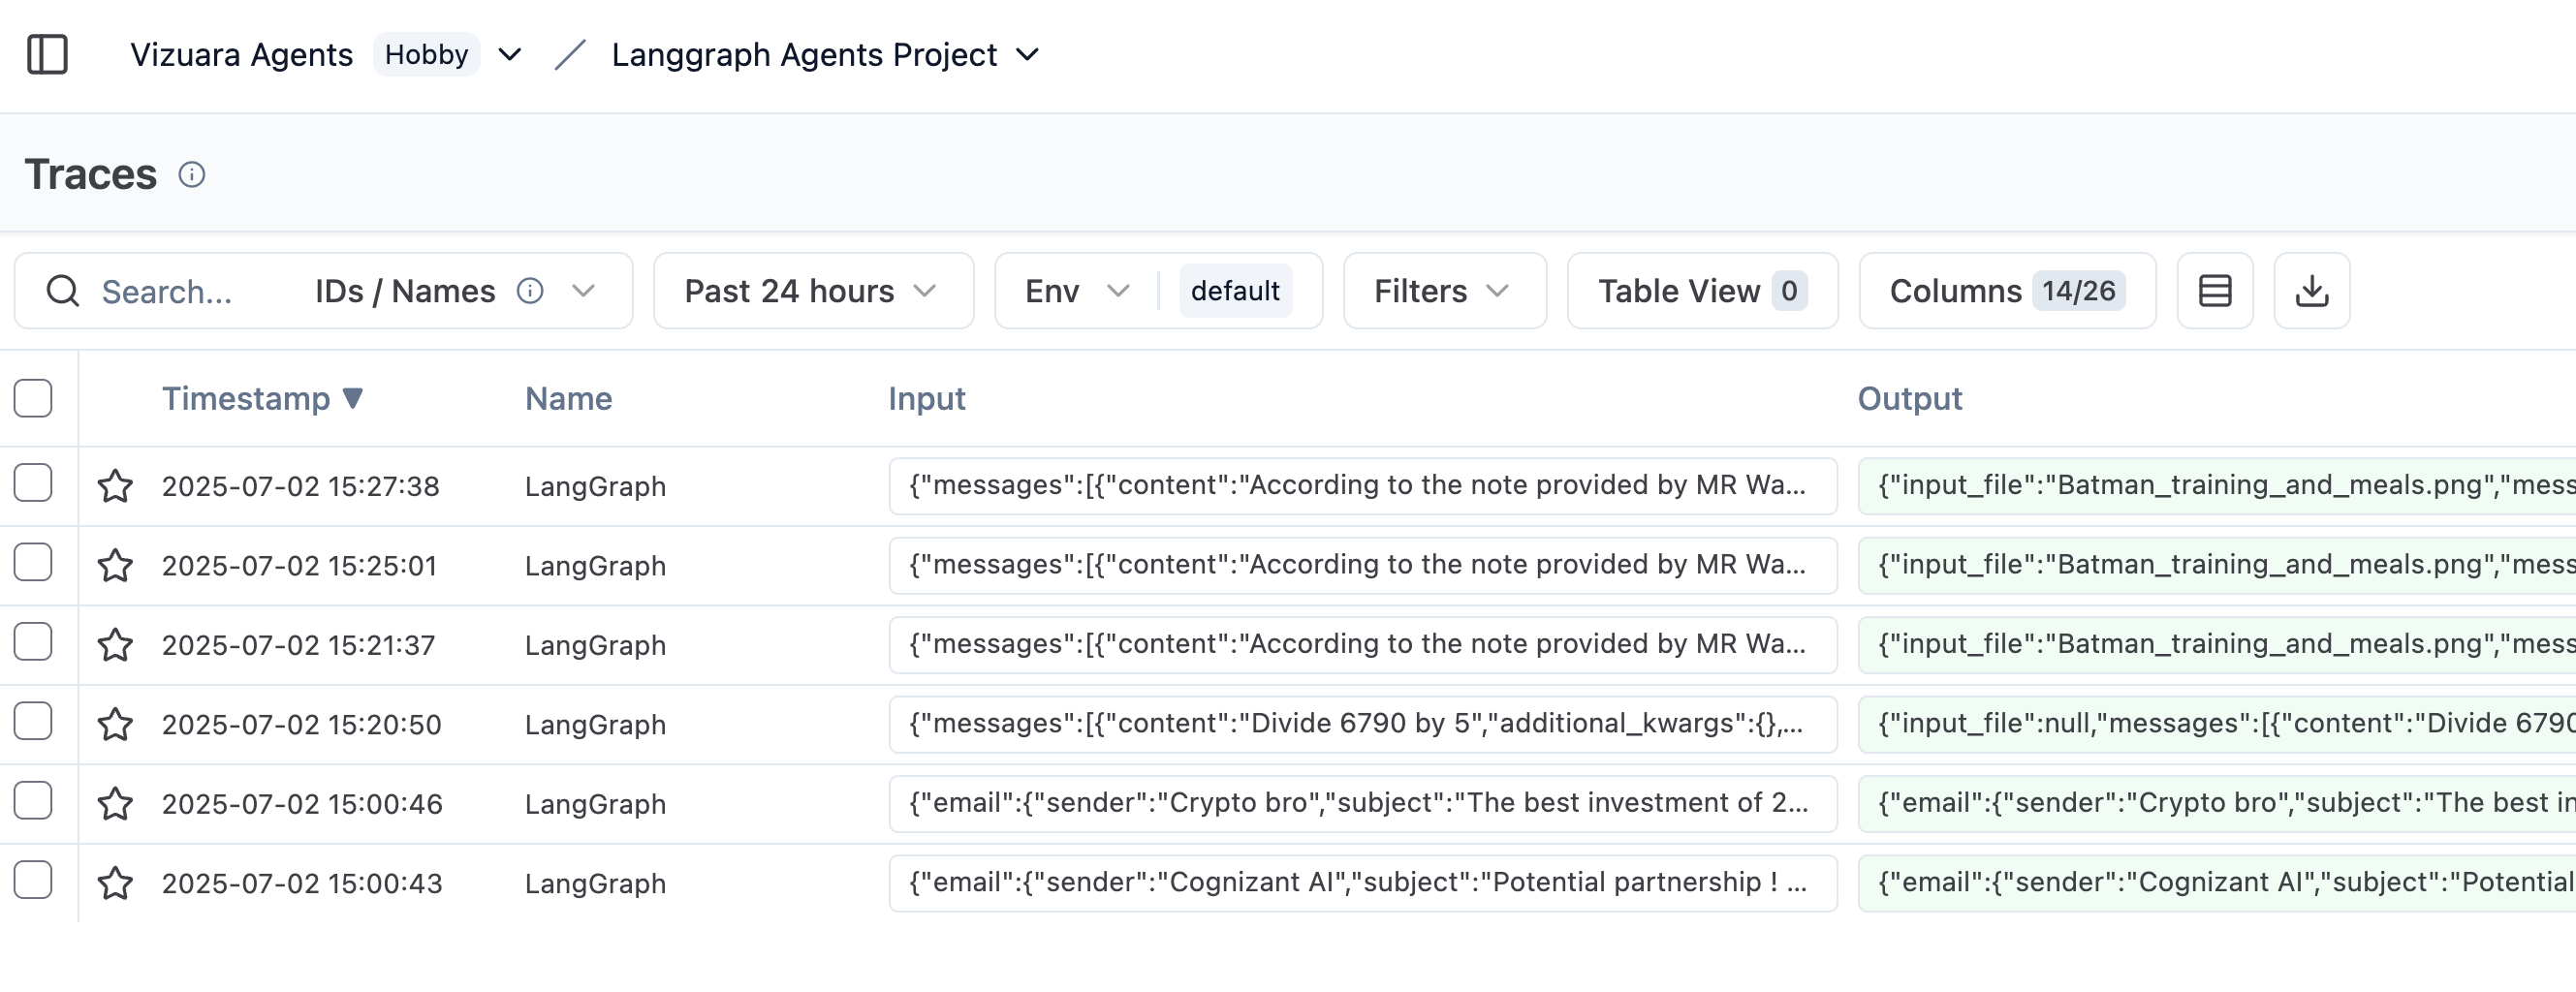
\includegraphics[width=\linewidth,keepaspectratio]{aiagents79}
		
		{\tiny (Ref: Vizuara AI Agents Bootcamp)}
				
        \end{center}    

\end{frame}

%%%%%%%%%%%%%%%%%%%%%%%%%%%%%%%%%%%%%%%%%%%%%%%%%%%%%%%%%%%
\begin{frame}[fragile]\frametitle{Tracing Agent Workflows with Langfuse}

        \begin{center}

        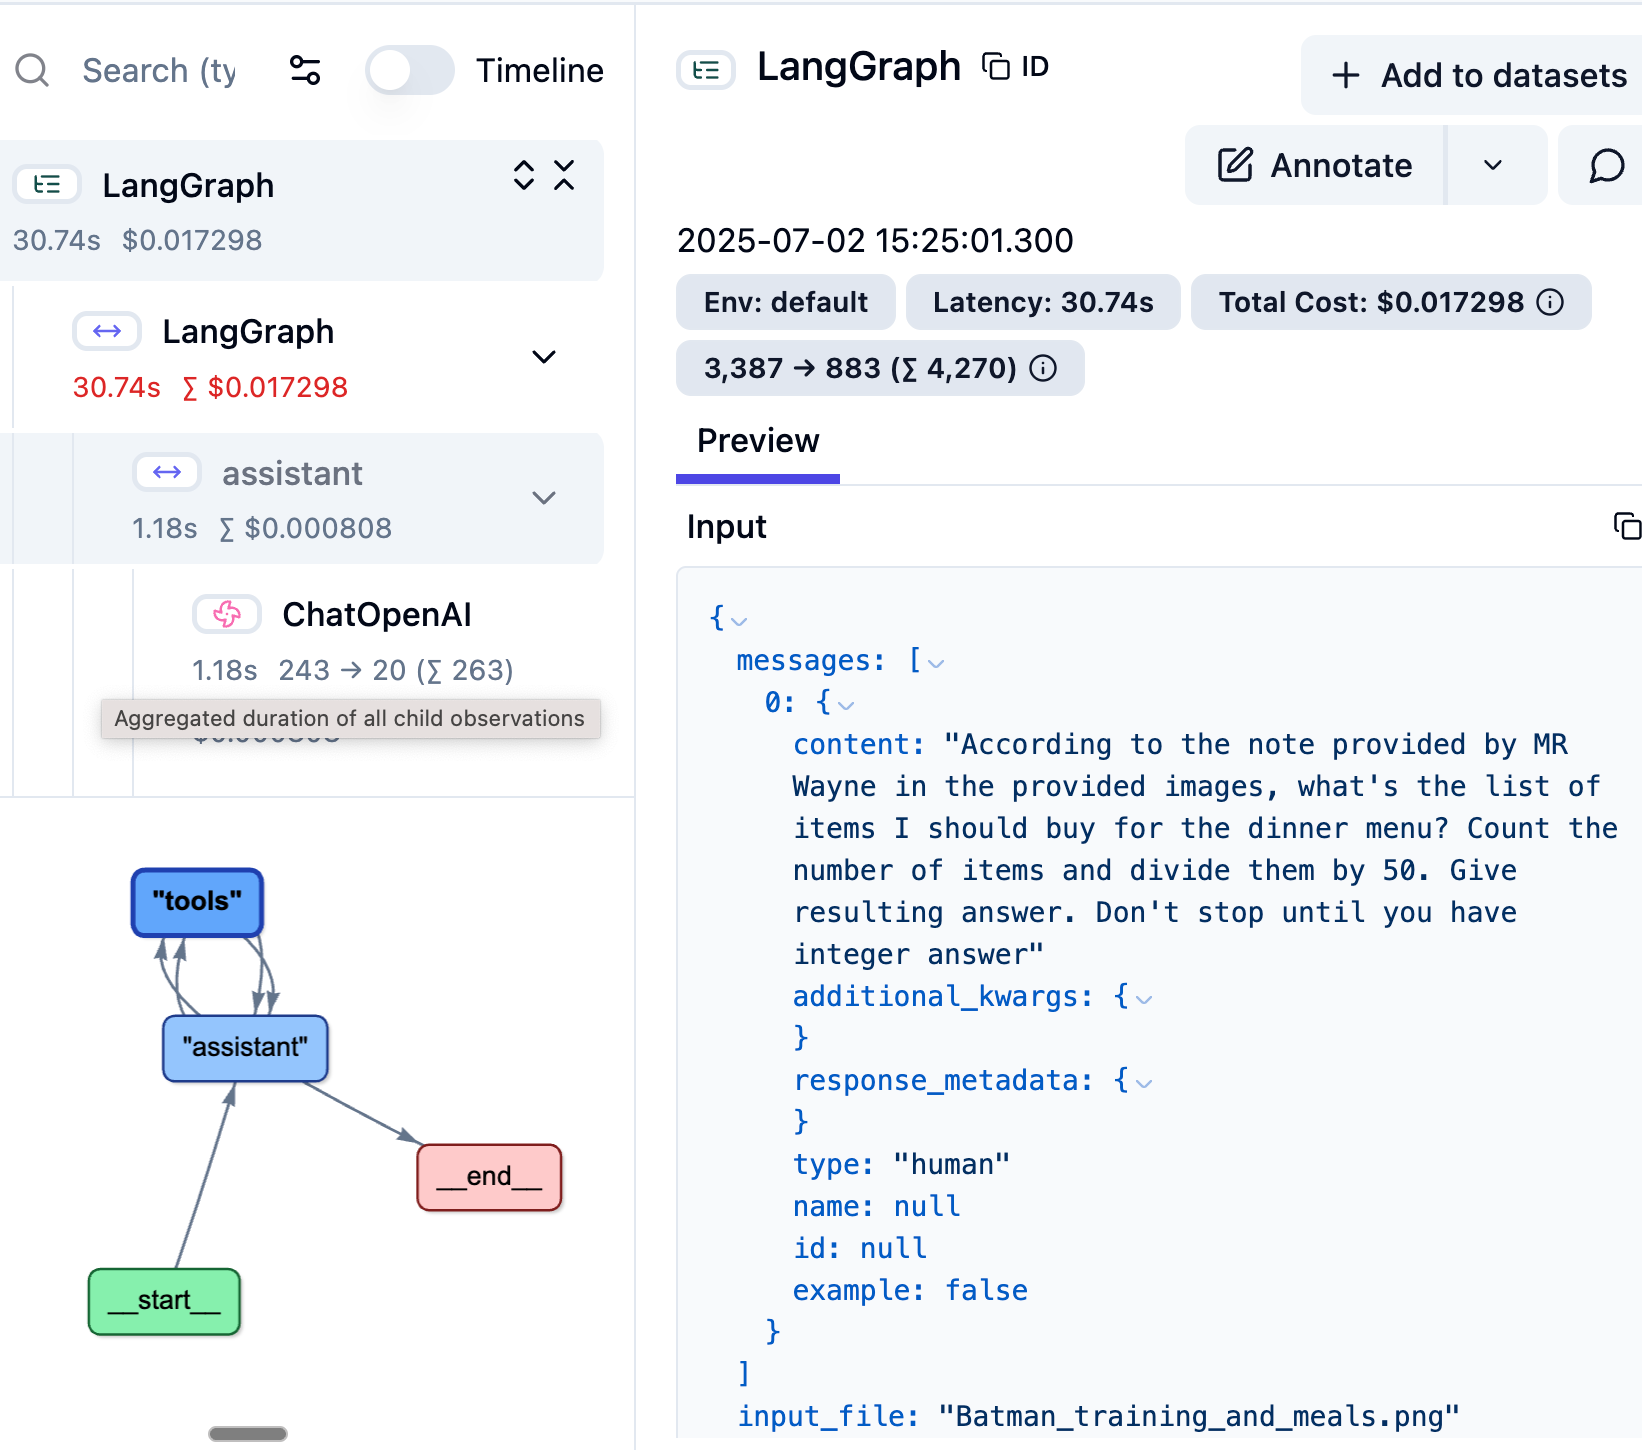
\includegraphics[width=0.7\linewidth,keepaspectratio]{aiagents80}
		
		{\tiny (Ref: Vizuara AI Agents Bootcamp)}
				
        \end{center}    

\end{frame}
